\documentclass[times, utf8, diplomski]{fer}
\usepackage{booktabs}
\usepackage{algorithmic, algorithm2e}    % for algorithm
\usepackage{fontspec}   % works with xelatex: for non-ASCII characters

\begin{document}

\thesisnumber{1763}

%\title{Evolucijske heuristike za pretragu prostora parametara napada umetanjem pogreške}
\title{Evolutionary Heuristics for Fault Injection Parameter Space Search}

\author{Antun Maldini}

\maketitle

\izvornik

\zahvala{}

\tableofcontents


% Questions for the introduction:
% -------------------------------
% what is the problem
% why is it interesting and important
% why is it difficult
% what have other people done
% what are the elements of our solution

% Structure:
% ==========
%   - motivation; twofold:
%      * stuff on cryptography, fault injection/analysis, EMFI in particular, which leads us to...
%      * the need for a better way to search the parameter space
% 
%   - related work: what have others done?
% 
%   - preliminaries:
%      * general crypto? but minimized to what's used
%      * EdDSA?
%      * SHA-3
%      * genetic algorithms
% 
%   - the THING:
%      * what was the plan & the setup
%         + the algorithm
%         + the baseline
%         + how we measure
% 
%   - results
%   - future work



\chapter{Introduction}\label{ch:introduction}
%The field of cryptography is a big one. As it is with most such fields, it
%abounds with rabbit holes: if you pick any one thing to know in detail, you'll
%end up going in progressively more detail, until you realize you're in deep
%enough that it's hard to describe your position to someone still at the
%entrance.
The field of cryptography is a pretty large and well-developed one. As it is
with most such fields, doing anything of worth means going down a rabbit hole
into progressively greater and greater detail, until it becomes hard to describe
where you are to someone standing on the surface. \\
This thesis is an attempt at covering one particular path down the rabbit hole.

Its structure is roughly this:
\begin{description}
    \item[chapter \ref{ch:introduction}] lays out the general motivation and
          the current state of the art;
    \item[chapter \ref{ch:prerequisites}] contains some technical prerequisites,
          covering evolutionary algorithms (and genetic algorithms in particular),
          fault injection, and SHA-3;
    \item[chapter \ref{ch:fault_injection}] presents the setup I've used and
          describes the parameter space and the problem at hand;
    \item[chapter \ref{ch:optimization}] deals with the optimization algorithm,
          the simulator built to aid experimentation, and the results obtained;
    \item[chapter \ref{ch:conclusion}] just wraps it all up, and presents
          directions for future improvements.
\end{description}


\section{Motivation}
Cryptography is ubiquitous; as technology keeps advancing, the normal functioning
of key infrastructure now depends on cryptographic algorithms. Billions of people
worldwide rely on it daily to protect not only commerce, but also their privacy.
But even with good cryptographic primitives, new attacks keep being discovered,
commonly against implementations.

Zooming into this picture for something more concrete, we may find a service
provider running attacker's code on the same machine as a vulnerable encryption
library, just waiting for a cache-timing side-channel attack; or a TLS
implementation that will curteously say when the padding is wrong, thus letting
an attacker steal a session; or perhaps, a smartcard that can be persuaded by a
carefully placed glitch in its power supply to give out its secret PIN.

Surely, no one would want their bank account emptied just because someone had
physical access to their debit card. But attacks like these do exists, and it's
this last case that's most relevant for this thesis: fault attacks.

They're usually not the easiest thing to do, and one part of \emph{why?} is
picking the right parameters. The core part of this thesis concerns finding
a good algorithm for picking the parameters, and (if possible) mounting a
successful fault attack.


%Implementation attacks do not aim at the weakness of an algorithm, but at the
%weaknesses in its implementation instead. Two well-known kinds of implementation
%attacks are side-channel attacks (SCAs) and fault injection (FI) attacks.
%Side-channel attacks are passive, non-invasive attacks where the device under
%attack operates within specified conditions and the attacker simply observes
%the physical leakages produced. Fault injection attacks are, on the other hand,
%active, more invasive attacks where the attacker inserts faults (glitches) in
%order to disrupt the normal behaviour of the algorithm.
%
%Side-channel attacks received a lot of attention in the last few decades where
%we saw successful exploitation of several side channels like timing~\cite{kocher-timing_attacks},
%power consumption~\cite{Kocher_SCA}, and EM emanation~\cite{10.1007/3-540-45418-7_17}.
%To use that information and deliver as powerful as possible attacks, researchers
%devised various strategies. What is especially interesting is that many of those
%strategies in the last few years are based on machine learning~\cite{lerman11, PicekHJLGJM17}
%and deep learning~\cite{CagliDP17}.
%%Although considering distinct attack scenarios and often various techniques,
%%all those papers have in common that they establish different use cases where
%%machine learning is a powerful attack technique.
%
%Somewhat surprisingly, when considering fault injection attacks, the situation
%looks much more straightforward. There are  several sources of glitches like
%laser pulses, electrical glitches, and electromagnetic radiation. A fault
%injection attack is successful if after exposing the device under attack to a
%specially crafted external interference, the device shows an unexpected behaviour
%i.e. a fault, which can be exploited by an attacker. Here, the challenge lies in
%selecting the appropriate parameters for a fault to succeed. If those parameters
%are not well chosen, the target will respond in a way that does not permit an
%actual fault analysis attack. When considering various sources of faults, there
%are different number of parameters and corresponding ranges. In general, the
%search space size of possible parameter values is large and relatively few
%points in the search space result in faults. Consequently, an interesting
%question is: how to find suitable parameter values or intervals, or more
%precisely, how to efficiently find the correct values in the search space?
%Surprisingly, the main options today are to use either random search or some
%sort of exhaustive search (since full exhaustive search is usually not possible
%the attacker will concentrate only in some regions with a certain precision,
%which we call here grid search). Analogously, if it is possible to make SCA
%more powerful by using machine learning (and more generally, artificial
%intelligence) one would expect the same to be possible with the fault injection.

%In this paper, we discuss how to use a special type of metaheuristics called
%genetic algorithms in order to find parameter values resulting in faults for
%electromagnetic fault injection. A somewhat similar research direction is
%followed in several papers~\cite{10.1007/978-3-319-08302-5_16, 6859734, 10.1007/978-3-319-21476-4_11}
%but there the authors consider power glitching, which is a much simpler case
%from the search space size perspective, and they attack the PIN mechanism in a
%smartcard. Here, we use the faults obtained via our technique to mount an
%algebraic fault attack on a SHA-3 implementation where we consider only pulsed
%EMFI and we have a total of 5 parameters. We emphasize that our version of
%search algorithm differs significantly from previous works as detailed in the
%rest of the paper. Finally, our code is available as an open source implementation~\cite{memfaultsGithub}.\\


This thesis is partly based on~\cite{paper_FDTC2018}, and hence reuses some
of the material.

\section{Related work}\label{sec:related_work}
While a lot of work has been done on fault injection itself (see
e.g.,~\cite{Kommerling, boneh_demillo_lipton, nsamwel_africacrypt, impeccable_circuits, FI_crowbars}),
very little of it concerns parameter optimization.

In~\cite{madau2017fault}, the authors develop an EMFI susceptibility criterion,
which they use to rank the points of the chip surface depending on how susceptible
they are to fault injection. The underlying assumption for the criterion is the
Sampling Fault Model, described in~\cite{ordas2015injection}. The Sampling Fault
Model could be summarized thus: faults are (mostly) induced by violating the
setup time constraint of D-type flip-flops, and the length of the time window
for fault injection does not depend on the clock frequency. (Early on during
development, I considered this might provide a way to substantially decrease
the search space size in the time-offset dimension; the practical problems of
synchronizing to the internal clock and the comparatively low time resolution
of the equipment ensured that this direction was not pursued.) The criterion
itself is a combination of Power Spectral Density (measuring emitted power at
the clock frequency) and Magnitude Squared Incoherence (measuring how linked
the emitted signal is to the data being processed), weighted with a configurable
parameter $a$ like so:
\[
    emfisc_{x,y} = \sqrt{a \cdot psdn_{x,y}^2   +   (1-a) \cdot incn_{x,y}^2}
\]
where $psdn$ and $incn$ are normalized Power Spectral Density and Magnitude
Squared Incoherence, respectively.


They use a grid scan (in the 2 spatial dimensions) to measure all the points
and rank them according to the criterion; a share $\alpha$ of the highest-ranking
points are kept for further scanning; the rest is thrown away.
They are able to reject over 50\% of the chip surface (75\% in their best case),
while keeping 80\% of the points causing faults. Figure \ref{fig:emfisc} shows
their coverage ratio -- the share of preserved faulty points -- dependent on $\alpha$.
However, note that by \emph{fault}, they mean \emph{any} perturbation of the
normal behavior of the algorithm.

\begin{figure}[htb]\label{fig:emfisc}
    \centering
    %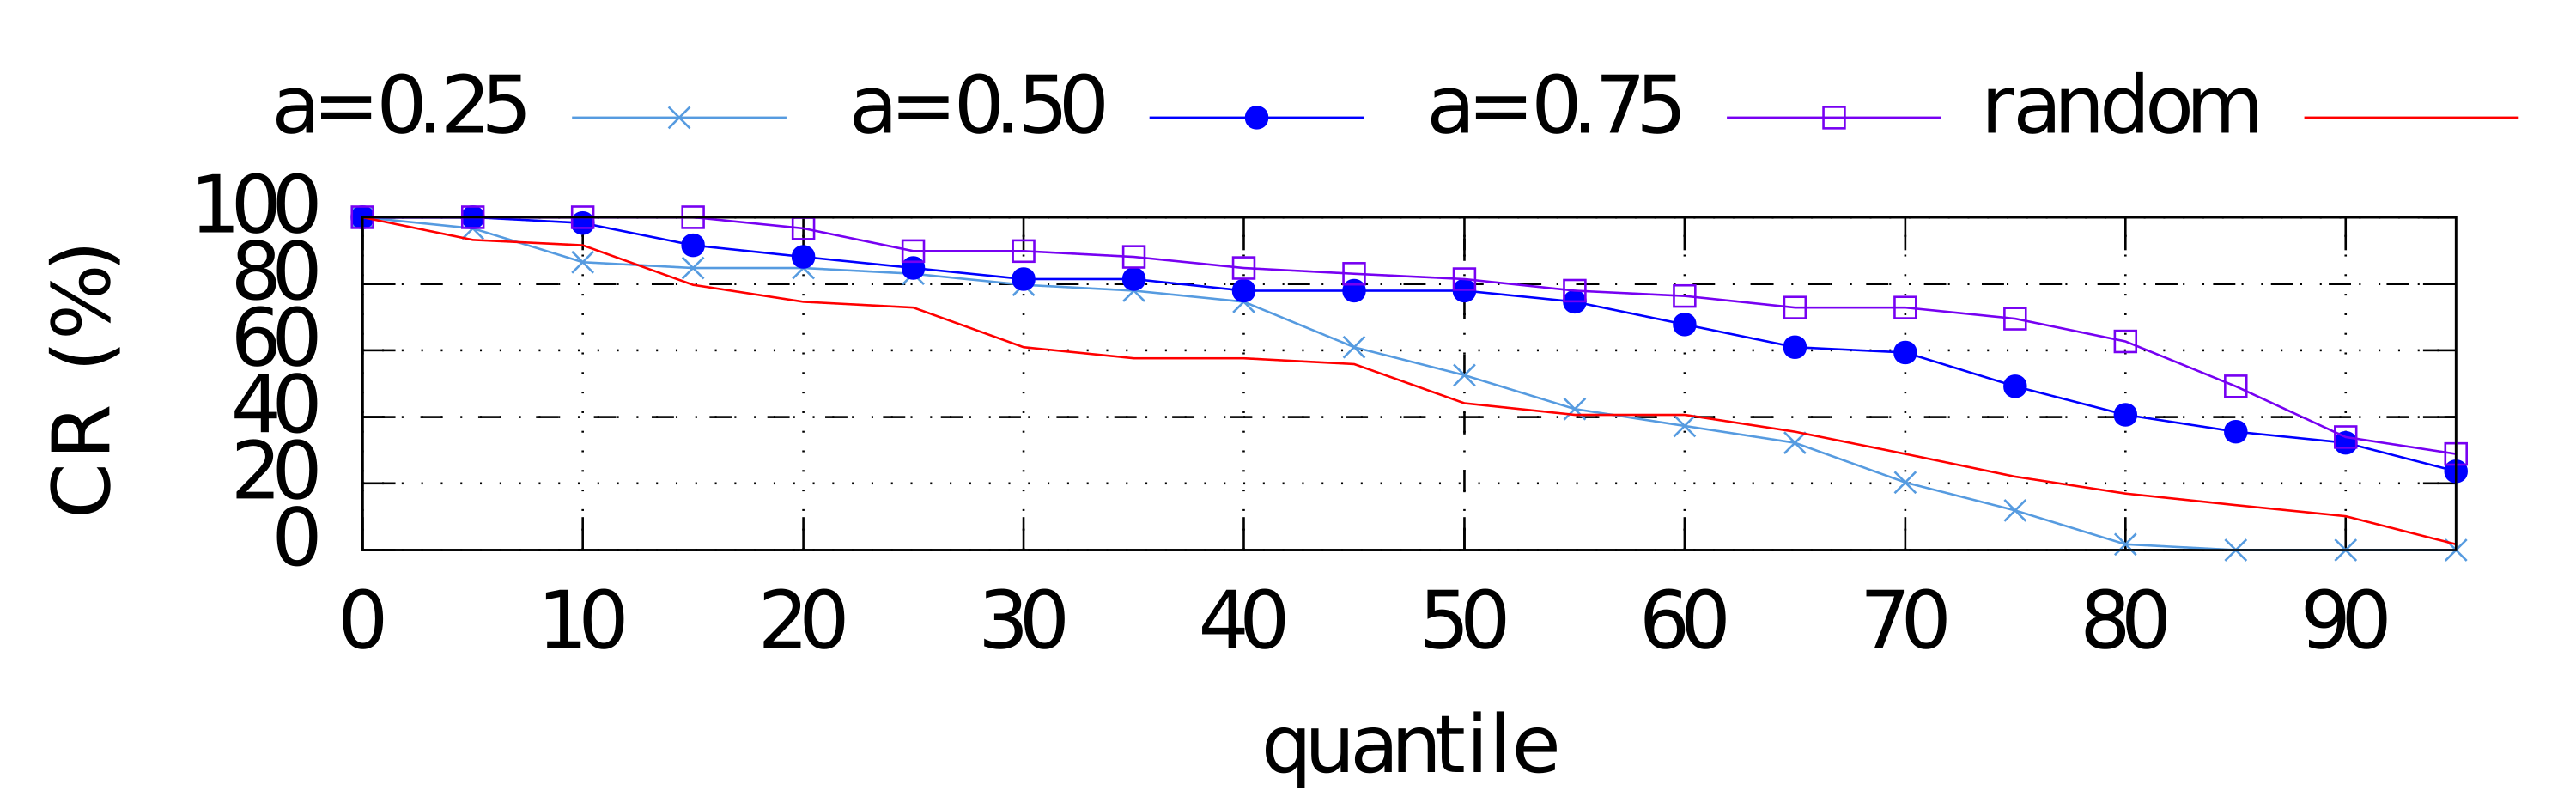
\includegraphics{images/emfisc.png}
    \caption{coverage ratio vs. $\alpha$ for EMFISC}
\end{figure}


In~\cite{GlitchItIfYouCan}, the authors use several different methods to the
problem of parameter optimization for supply voltage (VCC) glitching. They work
with 3 parameters: glitch voltage, glitch length, and time offset. They reduce
the dimensionality of the problem by splitting the search in two stages,
effectively solving a "2.5-dimensional" problem, so to say. In the first stage,
they look for the best (glitch voltage, glitch length) combination, i.e. the
most promising shape of the glitch. All parameters not explicitly specified
 -- in this case, time offset and the number of glitch repetitions -- are
set as random. In the second stage, 10 most promising (voltage, length)
combinations are tried at each point in the specified time range (which is
discretized into 100 instants), i.e. they perform a grid search in the time
offset dimension.

The methods are compared at the first stage -- random search, FastBoxing and
Adaptive zoom\&bound algorithms, and a genetic algorithm. While Adaptive
zoom\&bound comes out as the best strategy of these, the genetic algorithm
shows some promise. 
%This approach is a ``smart'' search in 2D with a grid search in 1D.

That work is extended in~\cite{FI_memetic} where the authors use a combination of
genetic algorithm and local search (called a memetic algorithm) in order to find
faults even more efficiently. The authors consider power glitching with 3
parameters and are interested in fast characterization of the search space.
%TODO: describe FI_memetic more closely?


The evolutionary algorithm developed for the purpose of this thesis builds on
the ideas of the latter two papers.



\chapter{Prerequisites}\label{ch:prerequisites}
In order to understand what was done and how, several things must be understood
first. These are:
\begin{enumerate}
    \item genetic algorithms, used here for optimization
    \item fault injection in general
    \item the SHA-3 hash function, which is exploited here using algebraic fault analysis
    \item algebraic fault analysis (AFA), which is used in conducting a real attack
\end{enumerate}


\section{SHA-3/Keccak}\label{sec:keccak}
In 2015., after a competition to choose the next SHA (Secure Hash Algorithm)
algorithm, NIST standardized Keccak~\cite{keccak_reference} as SHA-3.
Strictly speaking, SHA-3 is not one algorithm, but several, which all share
the same internal structure, and differ in a few parameters.

Its predecessors, SHA-1 and SHA-2, as well as some earlier algorithms which
weren't standardized but are still widely used (MD4, MD5), were based on the
Merkle-Damgård construction~\cite{merkle-damgard_reference}. Figure \ref{fig:merkle-damgard}
shows the general concept: the algorithm operates on blocks of data of size $B$.
There exists an underlying function $f$, called the \emph{compression function},
which takes $2B$ bits of input and produces $B$ bits of output. $f$ is essentially
a small hash function itself, but one with fixed-length input and output, which
the Merkle-Damgård construction uses to build a "big" hash function, with
arbitrary-length input. It can be proven that the "big" hash function will
be collision-resistant if and only if the compression function is
collision-resistant~\cite{}.

\begin{figure}[htb]\label{fig:merkle-damgard}
    \centering
    %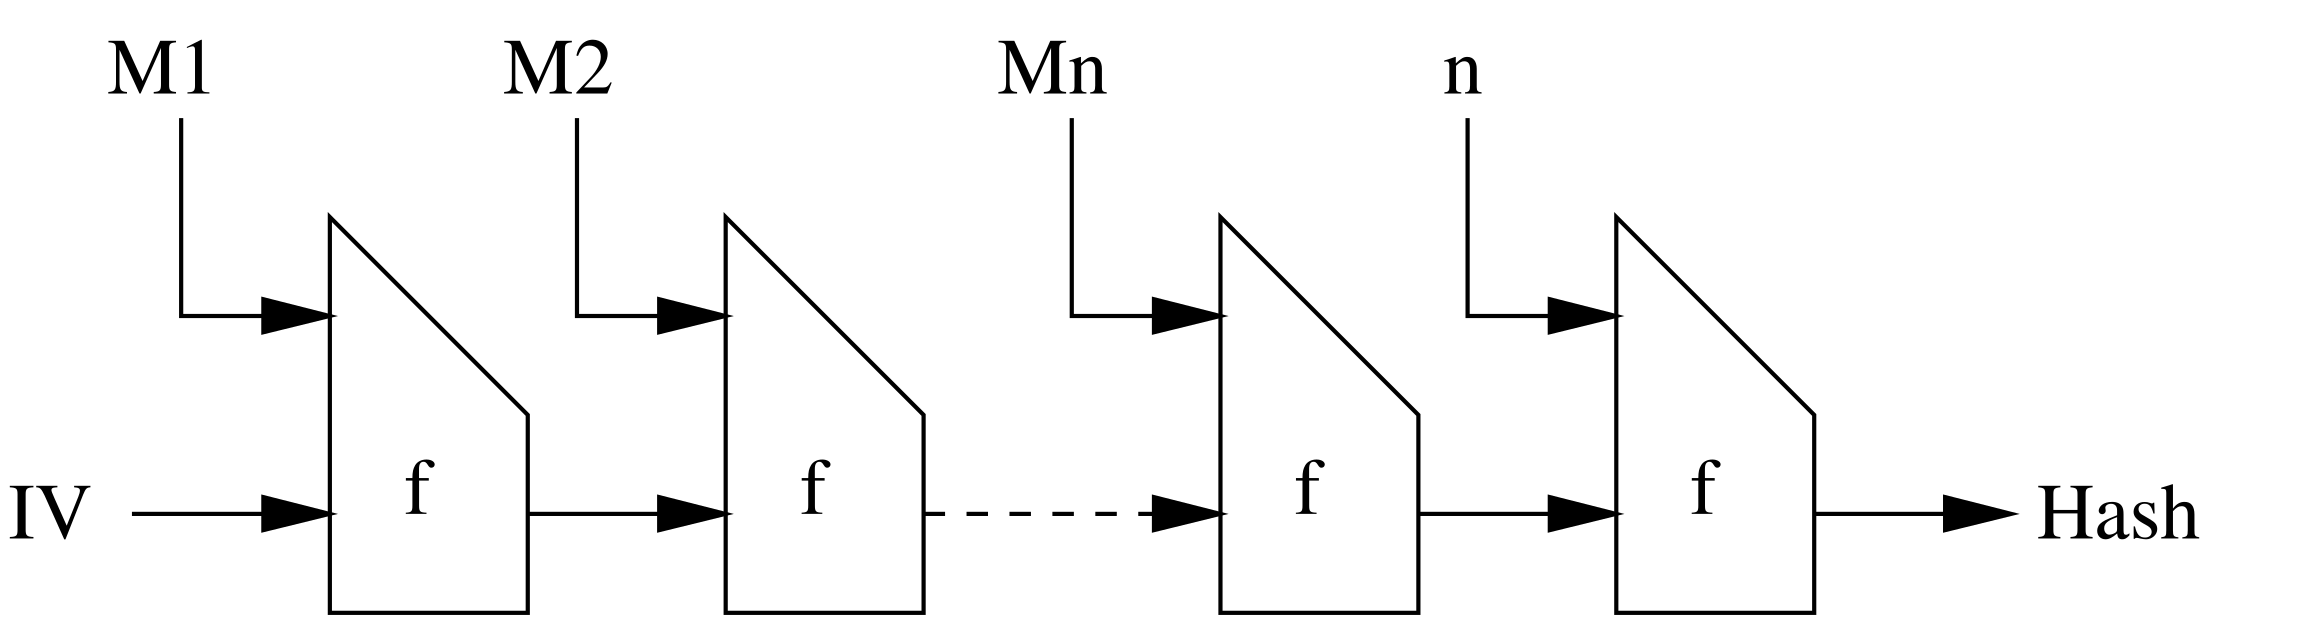
\includegraphics{images/merkle-damgard.png}
    \caption{the Merkle-Damgård construction}
\end{figure}


SHA-3, however, is based on a different construction called a \emph{sponge}.
It's called a sponge because unlike the Merkle-Damgård construction, which takes
an arbitrary amount of input and puts out a fixed-length output at the end, the
sponge can alternate between taking in chunks of input (\emph{absorbing}) and
putting out chunks of output (\emph{squeezing}); it has arbitrary-length output
as well as arbitrary-length input.
This is nicely illustrated in figure \ref{fig:sponge}.

%TODO: redo sponge description?

\begin{figure}[htb]\label{fig:sponge}
    \centering
    %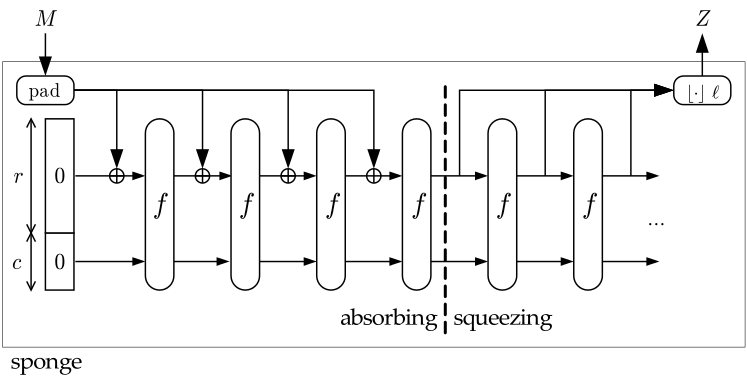
\includegraphics{images/sponge.png}
    \caption{the sponge construction}
\end{figure}

Another way to put it would be this: the Merkle-Damgård construction has a
compression function munging its internal state as well as chunks of input;
the sponge has a permutation mixing its internal state with chunks of input,
then mixing its internal state while spitting out chunks of output.

With traditional hash functions, security is expressed in terms of number of
output bits: a hash function with an $n$-bit output is supposed to have $n/2$
bits of security, i.e. the easiest attack has a complexity of $O(\frac{n}{2})$.
This corresponds to having a random oracle output $n$ bits, and attacking it
with the generic attack which relies on the birthday paradox.

But here, expressing its security in such a way obviously wouldn't make sense:
with an arbitrary-length output, it would mean that we can get an arbitrarily
high level of security merely by squeezing more bits out of the sponge.
Instead, this is expressed as a single parameter of the sponge construction.


\subsection{The Keccak-$f[b]$ permutation}
The central part of the sponge construction is the permutation.
Keccak uses the Keccak-$f[b]$ permutation, where $b$ is the size of its internal
state; this is also called the \emph{width} of the permutation. In the variant
standardized as SHA-3, $b=1600$.
We define two parameters: \textbf{rate} ($r$) and \textbf{capacity} ($c$),
with the constraint that $r + c = b$. The sponge will absorb $r$ bits of input
for each invocation of the permutation by XOR-ing the chunk of input with the
first $r$ bits of the internal state; the rate essentially tells us how fast
is the input processed. The last $c$ bits of the state are never directly
touched from the outside, and are never output; the output is taken again from
the first $r$ bits of the state. Capacity is the single parameter that sums up
the security level: $c/2$ bits for collision resistance, $c$ bits for preimage
and second preimage resistance. Several concrete SHA-3 hash functions are
defined with different capacities, denoted SHA3-$c$: SHA3-224, SHA3-256,
SHA3-384, and SHA3-512. Only the last one, SHA3-512, will be considered in
this thesis.


And now, for the definition of the relevant variant of the permutation itself:
the Keccak-$f[1600]$ is a sequence of operations on a 1600-bit state $A$, which
we can represent as a three-dimensional array of bits: $A[5,5,64]$. Coordinates
$x$ and $y$ should be taken modulo 5 and coordinate $z$ should be taken modulo 64.
If an index is omitted, this means the statement is valid for all values of the
omitted indices, e.g. $A_{(x,z)}$ refers to the column of bits having coordinates
of the form $(x,\ast,z)$. Figure \ref{fig:keccak_state} shows the notation used
for different parts of the state.

\begin{figure}[htb]\label{fig:keccak_state}
    \centering
    %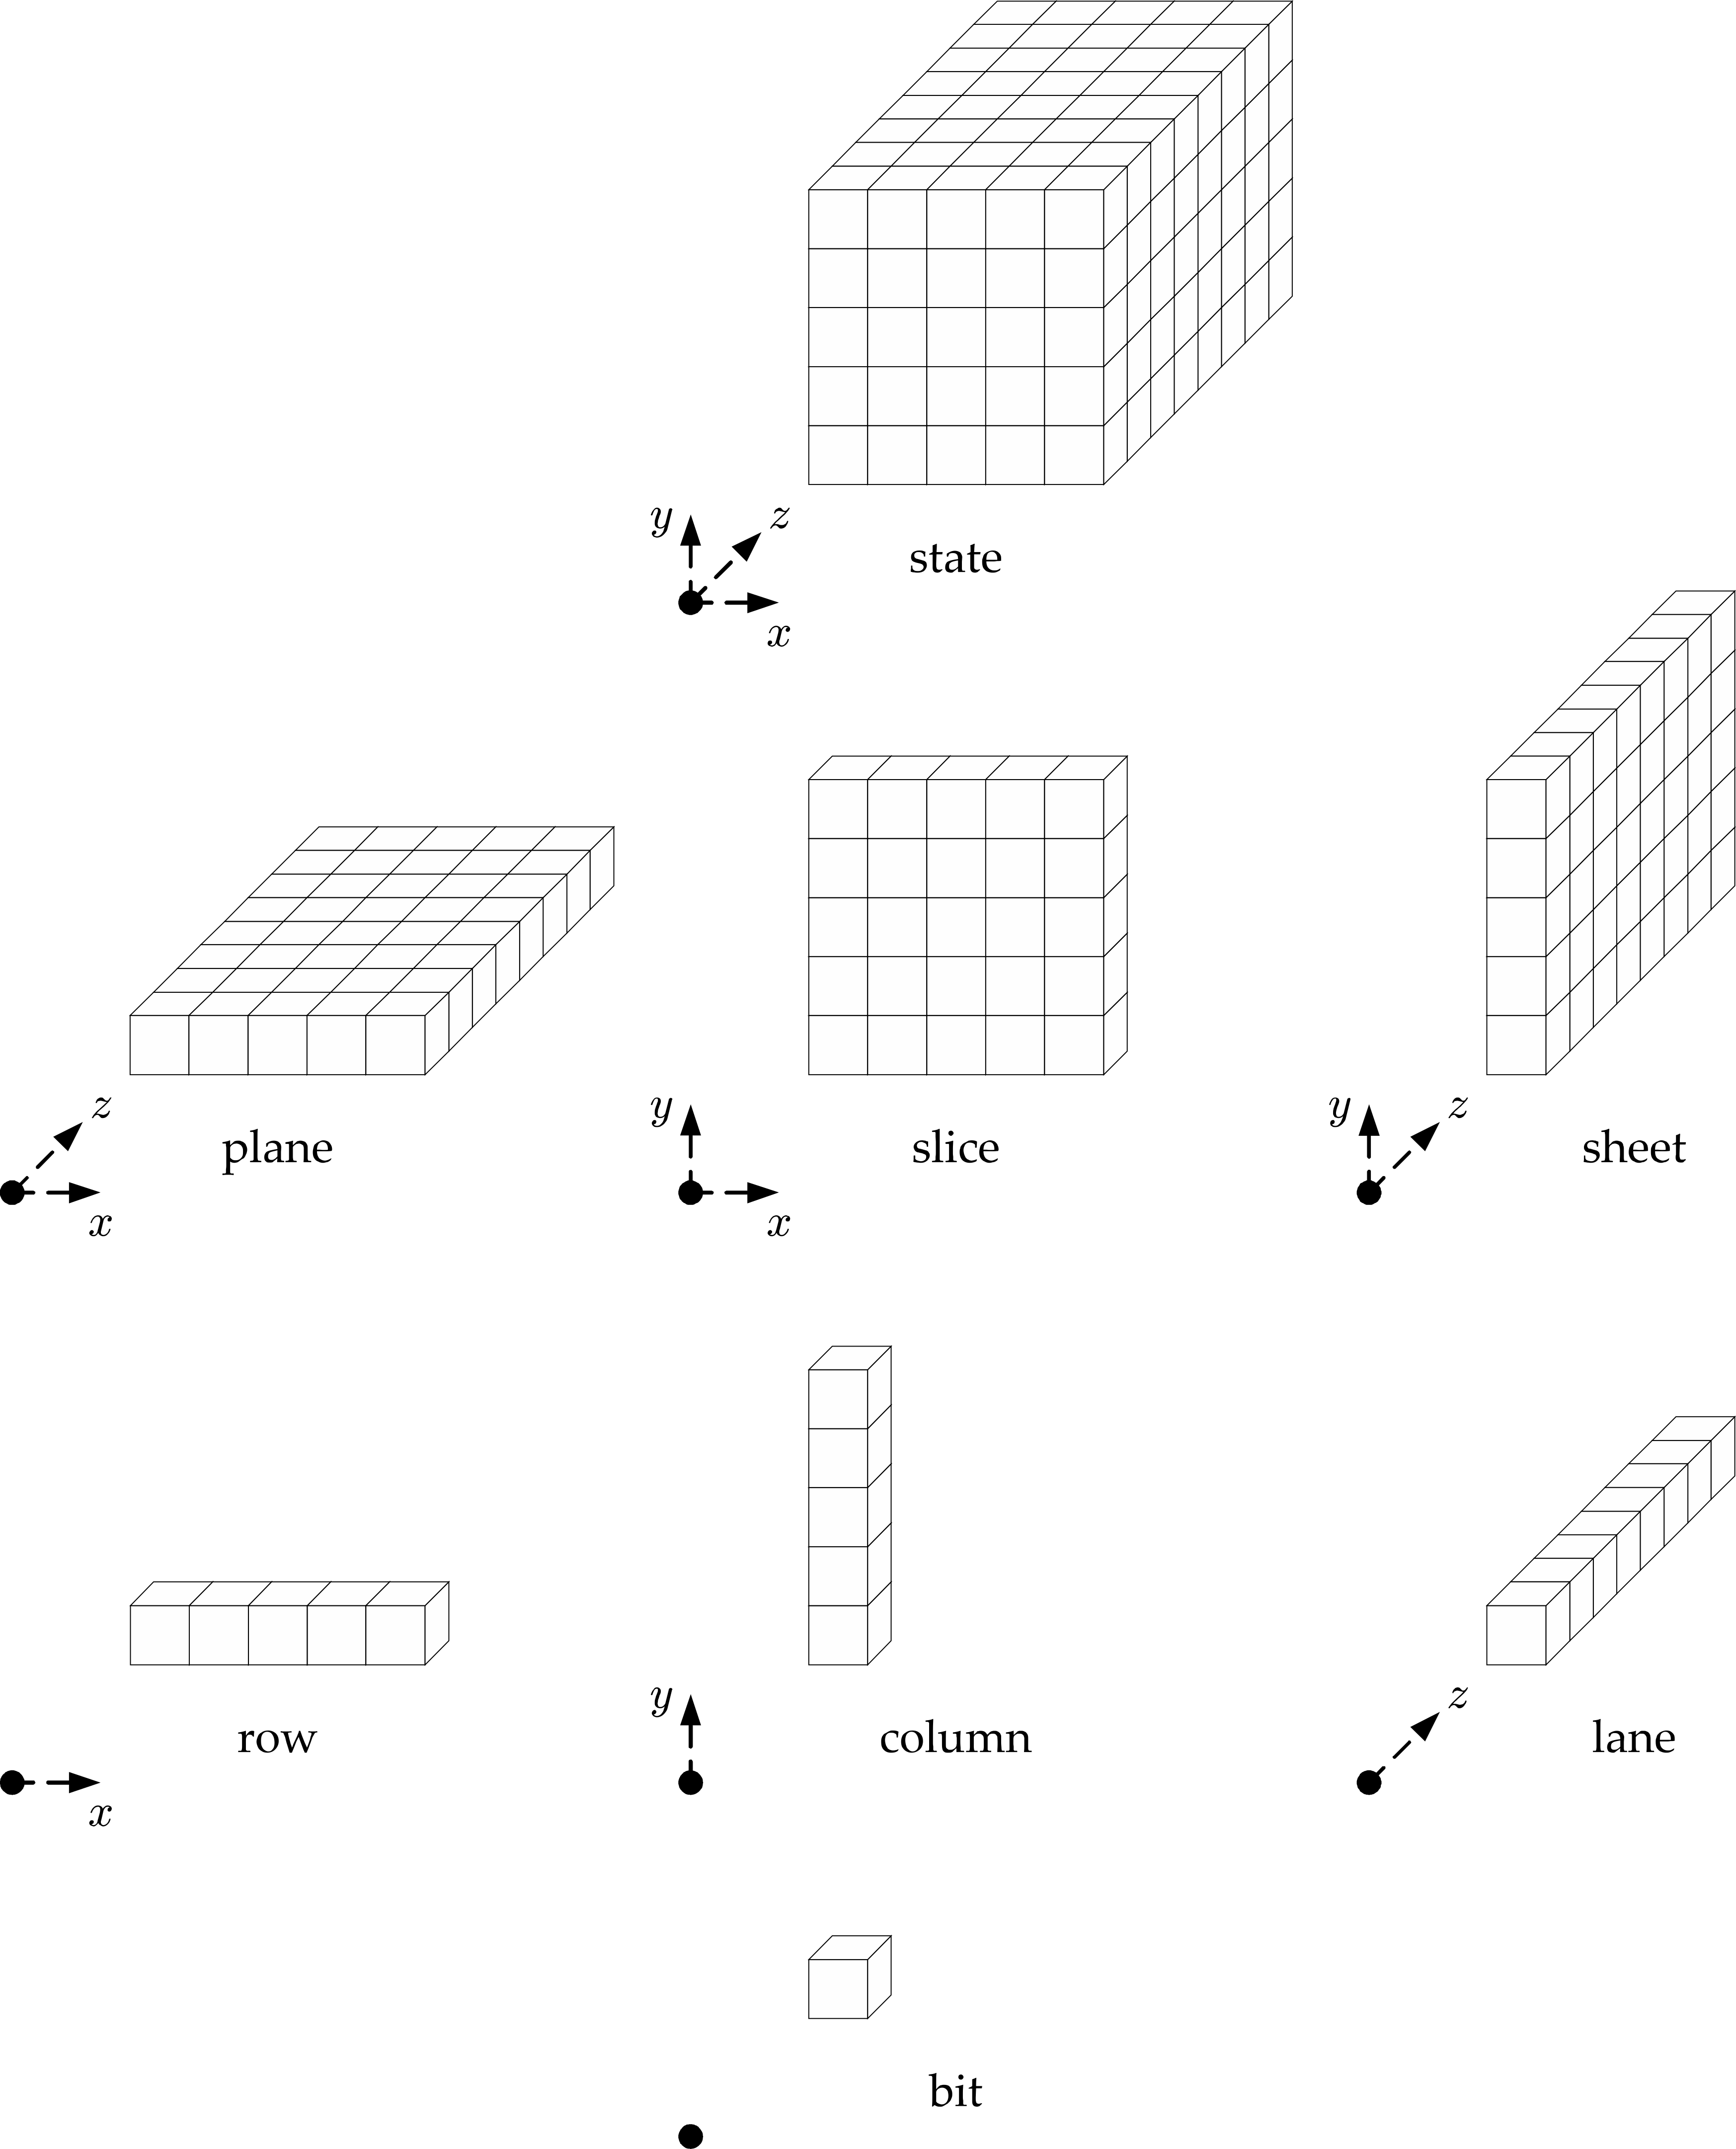
\includegraphics{images/keccak_state.png}
    \caption{notation for parts of the state array}
\end{figure}

The permutation is an iterated one, consisting of 24 rounds of $R$, where
\begin{equation*}
  R = \iota \circ \chi \circ \pi \circ \rho \circ \theta
\end{equation*}

is composed of five smaller phases:

$\begin{array}{rl}
  \theta:& C_{(x)} = \sum\limits_{y=0}^4 A_{(x,y)}\\
  &D_{(x)} = C_{(x-1)} + \text{rot}(C_{(x+1)},1)\\
  &A_{(x,y)} = A_{(x,y)} + D_{(x)}\\
  \pi \text{ and }\rho:& B_{(y,2x+3y)} = \text{rot}(A_{(x,y)}, r(x,y))\\
  \chi:& A_{(x,y)} = B_{(x,y)} + (B_{(x+1,y)} \times B_{(x+2,y)} + 1)\\
  \iota:& A_{(0,0)} = A_{(0,0)} + RC\\
\end{array}$\\

All operations are carried out in $GF(2)$, i.e. addition is bitwise XOR and
multiplication is bitwise AND. rot$(W,i)$ is a bitwise cyclic shift operation.
The constants $r(x,y)$ are rotation offsets. $RC$ is the round constant.
For more details, see~\cite{keccak_reference}.

%TODO: explain the phases properly


\section{Implementation attacks and fault injection}
Cryptographic algorithms that are perfectly safe in theory can be successfully
attacked in practice by attacking not the algorithm itself, but its implementation.
Any implementation which exists in the real world is a perfect black box: it can
be observed and interacted with outside of its nominal inputs and outputs.

Implementation attacks can be roughly divided into passive and active ones.

Passive attacks, also called \emph{side-channel attacks} (SCAs), do not interfere
with the execution of the cryptographic algorithm, but observe the effects the
implementation has on its surroundings, which leak secret information.
There are many: power consumption, electromagnetic radiation, timing, even sound. % TODO: add references?
These (unintended) side effects can be thought of as transmitting secret
information over a noisy channel, hence the name.

Active attacks, on the other hand, interfere with the cryptographic algorithm
somehow. They rely on inducing faulty behaviour, e.g. skipping instructions or
flipping bits, hence the name \emph{fault attacks}. They inject faults into the
operation of the algorithm, so the practice is called fault injection.
The common ones are:
\begin{itemize}
  \item operating the device outside of its safe operating range
        (too high/low temperature or voltage, over- or underclocking the device)
  \item injecting transient voltage spikes in the supply voltage (a.k.a. $V_{cc}$ glitching)
  \item exposing the board to an electromagnetic field, of a sinusoidal wave (harmonic EMFI)
        or short pulses (pulsed EMFI)
\end{itemize}

%TODO: rewrite this ^ paragraph better

Since only pulsed EMFI is considered here, in the rest of the text EMFI refers
to pulsed EMFI.


\section{Genetic algorithms}\label{sec:GAs}
Evolutionary algorithms (EAs) are metaheuristic optimization algorithms,
inspired by biological evolutionary processes and phenomena such as mutation,
recombination, and natural selection.
In a way, they simulate the natural process of evolution: a solution
(i.e. point in the solution space) becomes an individual in the population.
These "individuals" are then valued using a \emph{fitness function}; better
solutions are fitter individuals, with a higher chance of surviving and procreating.
Thus the objective function (which we are optimizing) gets mapped to the fitness function
and, over a number of generations, the evolutionary process takes care of the optimization.

Every generation, a number of individuals are selected from the population to
reproduce, i.e. to become parents; fitter individuals are given preference.
Those individuals are in some way combined to produce offspring (new solutions).
There is a small chance of mutations in the offspring: this allows the introduction
of new elements to the solution, which otherwise may not have ever been generated
from the initial population by just selection and reproduction.

After generating the offspring, the population is (whole or in part) replaced
by the offspring: the next generation.

The outline of an evolutionary algorithm is given below:
\begin{algorithm}[h]\label{algo:evolutionary}
    \begin{algorithmic}
        \STATE population := generate initial population
        \REPEAT
            \FOR{individual $\in$ population}
                \STATE evaluate fitness of individual
            \ENDFOR
            \STATE parents    := select ( population )
            \STATE offspring  := generate offspring ( parents )
            \STATE population := offspring

        \UNTIL{termination criterion met}

        \RETURN choose best individual ( population )
    \end{algorithmic}
    %\vspace{10pt}
    %\caption{evolutionary algorithm pseudocode}
\end{algorithm}

Mind that this is a fairly general outline.
The choice of selection and offspring generation makes all the difference.
Usually, however, offspring generation consists of two phases:
\begin{itemize}
    \item combining two (or more) parents to produce a child
    \item mutating the child with some probability $p$
\end{itemize}
It is not necessary for the entire population to be replaced in a generation.
A portion of the fittest individuals surviving across generations is called
\emph{elitism}; this could also be regarded as "cloning" the old solutions into
the next generation, so it fits in the outline given above.

This three-phase algorithm, when we represent the solution as a string of numbers,
is called a \emph{genetic algorithm} (GA).
In analogy to real life (though not exactly the same), this representation is
called the \emph{chromosome} (or \emph{genotype} or \emph{individual}; they're
interchangeable); multiple chromosomes are combined using \emph{crossover}
(or \emph{recombination}) to produce offspring.

However, what exactly falls under genetic algorithms and the exact lines between
GAs and other evolutionary algorithms can at times be a bit vague. That's okay,
since it's a metaheuristic we're talking about.
To instance this \emph{metaheuristic} into a \emph{heuristic}, we need to replace
these somewhat vague terms (selection, crossover, mutation, genetic representation)
with concrete ones. This is left up to the implementer.



\chapter{Fault injection}\label{ch:fault_injection}
One obvious prerequisite for doing fault injection is a physical device running
an actual algorithm to inject faults in. A cryptographic algorithm can be found
easily enough; a susceptible one, with a bit of literature review. A device to
attack, as well as the necessary equipment for glitching it, can be a bit harder
to find.

Section \ref{sec:setup} covers the physical setup used for the experiments;
section \ref{sec:parameters} presents the parameteters used, and section
\ref{sec:search_space} the big motivation for having a search at all.
Sections \ref{sec:assumptions} and \ref{sec:objectives} take care of
the implicit assumptions on the search space and our requirements for
the algorithm. Section \ref{sec:practical_considerations} covers some
practical implications of EM fault injection for the algorithm.

\section{Experimental Setup}\label{sec:setup}
For the target, a Cortex-M4 STM32F407IG (Riscure ``Pi\~{n}ata'') board was used,
running a C implementation of SHA-3. This implementation was taken from the WolfSSL
library~\cite{WolfSSL}, so as to have a real-world algorithm instead of a toy one.
The board communicates to a PC by a serial interface and is powered by an external
power supply (3.3V DC). For inducing an electromagnetic pulse, the Riscure EM probe
is used, as well as their VCGlitcher device that controls it. The board and the EM
probe are set up on an $XYZ$ table which moves the probe around in space.
The whole setup is controlled by code written in Python; for communicating with
the Riscure equipment, Python bindings for the VCGlitcher C API are used.
\footnote{
   Currently, due to the provided DLL being a 32-bit one, a 32-bit Python
   interpreter is required. This may change in the future.
}

Besides the serial interface, the board has a number of I/O pins which it can
toggle to high or low; the only one here used is the "trigger" pin. This pin is
used to signal to the VCGlitcher device that the cryptographic operation is in
progress; this is used as a reference point for injecting the fault. While this
slightly detracts from the realism of the attack, it greatly simplifies testing.
(It does not make much difference for the vulnerability status of the device,
since in real life the attacker only needs to spend more time figuring out the
timing.)

In the case that the board gets stuck in an illegal state after a glitch, it
needs to be reset. The only reliable way to reset this particular board is by
cutting its power, which can take a significant fraction of a second, depending
on the capacitors. A pause of 100ms was used for this.

The physical dimensions of the chip package are $24 \times 24$ $mm$.
Repositioning error of the $XYZ$ table is 0.05 $mm$, which gives a spatial grid
of at most $480 \times 480$. However, the limiting factor here is most likely
the size of the probe tip (and its internal coil), which is much larger.

%(TODO: compare to other people's more precise probe tips?)
All of these will, of course, vary depending on the chip and the equipment at
hand; even for different variants of the Piñata, the capacitors differ.
A more precise $XYZ$ table, a smaller probe (such as in e.g.~\cite{precise_probe_tips}),
or a smaller chip will give different spatial resolutions.


\section{Parameters}\label{sec:parameters}
There are multiple parameters to vary to affect the probability of causing a
fault: position of the probe tip (X, Y, and Z), pulse intensity, time offset
of the pulse, pulse duration, shape and angle of the probe tip, and pulse shape.

In the experiments conducted, only a subset of these are considered:
\begin{description}
  \item[position] -- two parameters (X and Y), since the distance from the board
        (Z) can be compensated by a change in intensity. The $(x,y,z)$ position
        in real space is mapped by the interfacing code to an $(x,y)$ position
        in the unit square $[0,1]^2 \in \mathbb{R}$.
  \item[glitch intensity] -- regulates the voltage of the pulse. The SDK manual
        suggests that it is a percentage of power used~\cite{RiscureVCGmanual},
        so it makes sense to map it to real values in $[0,1]$.
  \item[time offset] -- between 367 and 375 $ms$, because that is where the
        injection point must be, for the code we are running. The offset is
        encoded as an integer value (number of 2 $ns$ ticks).
  \item[number of repetitions of the pulse] -- a primitive form of pulse shape.
        This parameter is set to be in the (obviously, integral) range $[1, 10]$.
\end{description}

The pulse duration stays constant at a fixed value of 40ns. Similarly, the shape
and angle of the probe tip is not varied, since changing those cannot be easily
automated.



\section{Search Space Size}\label{sec:search_space}
One might wonder: why use a heuristic at all? What's wrong with a "dumb"
approach to parameter optimization? Let's consider the straightforward
approach: an exhaustive search.

The maximal spatial resolution, as I mentioned above, is $480 \times 480$ for
this particular setup; a better setup would have an even higher one. For the
time offset, the resolution is 2ns; for a reasonable range, I'll put the
interval between 367 and 375 microseconds, since this was measured as the
interval containing the fault injection point -- this gives us a total of
4\,000 different values; for the glitch intensity, there's really no good rule
for determining the smallest meaningful increment, but a 1\% increment seems
a fairly reasonable (if conservative) estimate based on visual estimates of
the results, which would give a range of 100 values; the repetitions parameter
in range $[1,10]$ gives an extra 10 values.

The total size is therefore $480*480*4\,000*100*10\approx 10^{12}$.
At $\approx0.16$ seconds per measurement, and five measurements per point, this
results in 29\,203 years to conduct an exhaustive search. Even if completely
ignoring everything but X, Y, and offset, an exhaustive search would still
take 29.2 years to finish.


\section{Some assumptions}\label{sec:assumptions}
From the viewpoint of the optimization algorithm, the device should be as close
as possible to a black box. That is to say, the algorithm should not have built-in
assumptions that would be broken by running it for another device or cryptographic
algorithm. However, I do make several assumptions:
one, the objective function is not a golf-course. In a golf-course function, the
gradient in the fitness landscape doesn't lead to optimal solutions, which tend
to "pop out of nowhere", all of a sudden. Given the nature of EM glitching, the
transition between different kinds of behaviour should be reasonably gentle; the
reasoning behind it is that a very weak EM pulse will not affect the target at all,
and we will observe normal behaviour. Conversely, a very strong EM pulse will
completely dishevel its operation and even potentially damage it. So, we should
expect faulty behaviour to occur somewhere between those two extremes, i.e.,
along the class border.

Additionally, offset ranges (min to max offset) are set by the user,
based on a rough expectation of the duration of the cryptographic algorithm.

Usually, the objective function guides the optimization algorithm towards better
solutions, and the algorithm ends when it finds the best one. Here, we don't want
just a single "best" solution since not every fault that's found will also be
exploitable, and there are situations where more than one are required, so the
aim is to obtain multiple solutions.


\section{Objectives}\label{sec:objectives}
The requirements for this optimization algorithm are:
\begin{description}
    \item[Good coverage of the parameter space] -- since we do not know where the
          exploitable faults are located, we need to explore the search space efficiently.
    \item[Speed] -- we require the algorithm to be fast in finding the faults, otherwise
          there is no advantage of using it when compared to random search, for instance.
\end{description}

These two requirements somewhat conflict with each other. Because most of the
parameter space is useless (i.e., has no faults), covering enough space to be
reasonably secure we did not miss anything important means potentially wasting
a lot of measurements.

Next, the terminology used when discussing the search and possible outputs of the algorithm.
A point is a distinct set of parameters, i.e., a point in the parameter space.
A measurement is the result of a single attempt at glitching the target with those parameters.

Each point is measured five times, since trying the same parameters multiple
times does not necessarily always yield the same response.

When counting the faulty measurements, we distinguish between:
\begin{enumerate}
    \item the total number of faulty measurements,
    \item the number of distinct faulty responses (i.e., ``unique faulty measurements'').
\end{enumerate}

The difference is that if a measurement results in a before-seen faulty output,
the second one will not be counted this second time around.
To better illustrate this: say we find a set of parameters $S_1$, which is
measured five times, with one of the measurements giving a faulty output $h_1$.
Later, we find some other set of parameters $S_2$ that results in two faulty
outputs, $h_1$ and $h_2$. Out of the ten measurements performed in total, three
of these are considered faulty, but with only two distinct faulty responses:
$h_1$ and $h_2$, since $h_1$ is not counted twice.
For the purposes of exploitation, the number of distinct faulty responses is
more interesting.

We classify the board response in one of the following classes:
\begin{description}
    \item[NORMAL]   -- for normal behaviour, meaning the board performs as if it wasn't glitched
    \item[RESET]    -- the board did not reply at all, requiring a reset to restore to normal operation
    \item[SUCCESS]  -- the board produces an output/ciphertext/signature/hash different than the correct one
    \item[CHANGING] -- for each point, 5 measurements are performed. If all measurements are in the
                       same class, the point is put into one of the first three classes; otherwise
                       it goes into the CHANGING class.
\end{description}


\section{Practical Considerations}\label{sec:practical_considerations}
Commonly, optimization algorithms (and nature-inspired metaheuristics in
particular) rely on a large number of iterations. Another assumption usually
made is that the evaluation of possible solution points is uniform. Here,
however, we have expensive measurements, where the cost of evaluation depends
not only on the properties of the point itself, but also the context of its
evaluation.
%Although our algorithm consists of genetic algorithm and local search, we denote
%it often as genetic algorithm but we always consider it to have also local search
%phase. We do not call our technique a memetic algorithm since the GA and local
%search phases are separated.
%
When considering EM fault injection, the probe tip has to physically move to
a different point. To do this with sufficient precision requires a non-negligible
amount of time -- the exact amount varies depending on the setup, but it can be
up to several seconds per measurement. In comparison, a reset requires just a
fraction of a second (for this board, $\approx100$ms to do it reliably). The
measurement part itself is even faster -- 30ms or less. Thus, the order in which
points are evaluated matters.

Even with an optimal routing for any batch of $N$ points, splitting the
evaluation into more batches means more time wasted. For population-based
algorithms, this translates to small population sizes being less efficient
than large ones. Additionally, we may want to get a glimpse of the results
even before the scan is finished, especially for long-running scans. In the
case of a random or grid scan, this requires splitting the scan into batches
where each covers more or less the whole parameter space, since scanning points
in the optimal (or nearly-optimal) order results in uneven coverage: as a
general rule, a segment the shortest Hamiltonian path from any given starting
point will not evenly cover the $(X,Y)$-plane, but instead a small part of it.

%TODO: calculate exactly how much less efficient?



\chapter{Optimization}\label{ch:optimization}
Now, to deal with the optimization itself.

Since EM fault injection is an \emph{expensive} optimization problem, I created
an emulator of the board to respond in its stead. While most scans were in the
end done on the actual Piñata board, the emulator helps to predict and visualize
behaviour of different algorithms (or the same algorithm, but differently
parametrized) over multiple runs, with only a fraction of the runtime cost.
However, we can only expect this if the behaviour of the emulator closely
matches that of the board. This poses a problem: how do we achieve this?
Obviously, without modeling the chip itself (which would be a large problem
in and of itself), the emulator must rely on samples of the objective function.

The straightforward solution would be to exhaustively sample the parameter space
and use a lookup table, but as mentioned in section \ref{sec:search_space}, it's
impossible in terms of time, and very hard in terms of space ($\approx 5 \cdot
10^{12}$ measurements!). What \emph{is} possible, however, is a lower-resolution
grid scan, with interpolation between points. This was, in fact, performed: the
largest of these is a grid scan with $1/40$ resolution in the XY-plane, $1/20$
resolution in the intensity dimension, 9 offset values (from 367μs to 375μs,
with 1μs step), and with repetitions set to 1. This gives $41 \times 41 \times
21 \times 9 = 317709$ points; with an average of 1.125s per point, around 100
hours, or a bit over four days. Given that this is a grid scan, it greatly
simplifies storage and nearest-neighbour lookup: caching it as a bare NumPy
array in a binary file takes up less than 3MiB of space, the loading takes
just a fraction of a second, and once in RAM, the lookup is as trivial as it
gets. This is relatively easy to extend to k-nearest neighbours.

Another variant, made convenient by the availability of a number of scans of the
parameter space, would be to abandon the notion of a regular grid, aggregate all
those scans, and use that as the underlying information.

%TODO: more information on this?

In any case, the emulator will be intrinsically limited due to being bound to
actual data.


\section{Algorithm}

TODO: write up the algorithms used, adapt the main GA writeup

%Despite the fact that we use genetic algorithms like some previous
%works~\cite{10.1007/978-3-319-08302-5_16, 10.1007/978-3-319-21476-4_11},
%our custom made algorithm is quite different. We discuss the specifics of our
%design in the following paragraphs. Our algorithm has several parameters to be
%determined. We selected those values on the basis of our tuning experiments and
%recommendations from~\cite{10.1007/978-3-319-08302-5_16,10.1007/978-3-319-21476-4_11}.
%
%
%More in detail, our algorithm consists of two separate phases as follows:
%\begin{enumerate}
%    \item The first phase is a genetic algorithm where we run it for  20 generations with population size 50.
%    \item Only when the genetic algorithm is done, we start with the local search, which takes 10 randomly chosen points in neighbourhood of each SUCCESS point. Note that this is a significant difference from related works where both GA and local search worked at the same time. We opted first to concentrate on exploration aspect -- GA (to explore various regions of the target) and only after that on exploitability aspect -- local search (to concentrate on more promising regions). Naturally, GA itself has also exploitability component that is especially manifested in the crossover operator but we also designed a custom made crossover operator that promotes exploration perspective.
%\end{enumerate}
%
%%Fitness values are set according to the class: SUCCESS has the highest fitness (10), followed by the CHANGING,
%%then RESET (5), and finally, NORMAL (2).
%%CHANGING points' fitness depends on its underlying measurements: a mix of NORMAL and RESET points
%%is somewhat better than all RESET or NORMAL point, but having SUCCESS points individual measurements
%%moves the fitness close to an all SUCCESS point. We calculate the fitness of a CHANGING point in the following way:
%%\begin{eqnarray}
%%    fitness_{CHANGING} = 4 + 1.2*N\_SUCCESS +\\\nonumber 0.2*N\_NORMAL + 0.5*N\_RESET.
%%\end{eqnarray}
%%Here, factors 0.2 i 0.5 are chosen in analogy to the values for NORMAL and RESET (which are 2 and 5) while, the rest of the factors are selected for the scaling reasons.
%%For example, 4 NORMAL and 1 RESET point give fitness 5.3, which is higher than the fitness of a RESET point (with all 5 RESET measurements). Similarly, 4 SUCCESS and 1 RESET point give fitness 9.3, which is lower than the fitness of SUCCESS point (with all 5 SUCCESS measurements).
%
%
%\subsubsection{GA Phase}
%Our algorithm begins with a genetic algorithm that runs for $N$ generations and has a population of $M$ individuals. 
%The initial population is selected uniformly at random within parameter ranges.
%We aim to maximize the fitness value, which corresponds to having as much as possible SUCCESS points.
%
%The first phase of GA is selection and we use roulette wheel selection. There, the fitness function assigns a fitness to possible solutions or chromosomes. This fitness level is used to associate a probability of selection with each individual chromosome. Those individuals that have better fitness are also proportionally more likely to be selected.
%We also use elitism where the elite size equals 1. This means that the best individual cannot be replaced by some other individual (e.g., mutated offspring). We also experimented with $3$-tournament selection as used  in~\cite{10.1007/978-3-319-08302-5_16,10.1007/978-3-319-21476-4_11} but we found it to be too restrictive, i.e., to promote too fast convergence resulting in obtaining solutions from only a small part of the search space.
%
%%\subsubsection{Binary search phase}
%%One of our assumptions was that the objective function was not a ``golf-course'',
%%i.e. that it has reasonably smooth transitions between classes. With this, we would
%%expect to find one or more 'blobs' of RESETs, wrapped in a thin layer of JUSTRIGHTs
%%and CHANGINGs, and the rest covered in NORMALs. Since this border area is where we
%%want to focus, we first need to more precisely locate it and map it out.
%%
%%This phase does exactly that: for each such blob, it picks a point somewhere inside it
%%(ideally its centroid). It then randomly picks a number of NORMAL points outside of it,
%%and performs a binary search to detect where the line connecting such a pair of points
%%intersects the inter-class border.
%
%After the selection phase, we run crossover. Note, this version of a crossover promotes explorability and it enables GA to traverse large parts of the search space.
%The pseudocode for crossover is given below:
%\begin{algorithm}
%    \algsetup{linenosize=\tiny}
%    \small
%    \begin{algorithmic}[1]
%        \FOR {$all \ parameters$}
%        \STATE $child = uniformly \ random \ value \ in \ the \ range [parent1, parent 2]$
%        \ENDFOR
%    \end{algorithmic}
%\end{algorithm}
%
%Finally, the last step is the mutation operator that works as follows:
%\begin{algorithm}
%    \algsetup{linenosize=\tiny}
%    \small
%    \begin{algorithmic}[1]
%        \FOR {$param \ in \ [x, y, intensity]$}
%        \STATE $random = random \ value$
%        \IF{$random > p\_mutation$}
%        \STATE $r = uniform \ random \ from \ interval \ [-0.5, 0.5]$
%        \STATE $param = param + r$
%        \ENDIF
%        \ENDFOR
%        \STATE $random = random \ value$
%        \IF{$random > p\_mutation$}
%        \STATE $r = uniform \ random \ from \ interval \ [-0.5, 0.5]$
%        \STATE $offset <- offset + r * OFFSET_RANGE$
%        \ENDIF
%        \STATE $random = random \ value$
%        \IF{$random > p\_mutation$}
%        \STATE $repetitions = random \ integer \ from \ [1, 10]$
%        \ENDIF
%    \end{algorithmic}
%\end{algorithm}
%
%The mutation rate $p\_mutation$ is set to 5\%.
%In the case the parameter gets out of its ranges, it is clipped to the edges of its range.
%
%
%\subsubsection{Local Search Phase}
%After GA is done, we focus local search on the promising parts of the explored search space: the space around the intersection points (i.e., places where class values change), and the space around any faults we've already found.
%We define the neighbourhood of a point as a cube centred in it, with edge length
%equal to 0.02. By length of 0.02 in parameter space, we mean 2\% of the range of that parameter.
%Parameters $x, y$, and intensity are all within the range $[0,1]$.
%For offset, it's 2\% of OFFSET\_RANGE (which is OFFSET\_MAX - OFFSET\_MIN).
%To determine the distance of values, we use the Euclidean distance.















\chapter{Conclusion}\label{ch:conclusion}
Conclusion goes here, as well as future work.

\bibliography{literatura}
\bibliographystyle{fer}

\begin{sazetak}
Sažetak na hrvatskom jeziku.

\kljucnerijeci{Ključne riječi, odvojene zarezima.}
\end{sazetak}

\engtitle{Evolutionary Heuristics for Fault Injection parameter Space Search}
\begin{abstract}
Abstract.

\keywords{Keywords.}
\end{abstract}

\end{document}
